% Name: Adjacency list
% Description: A four-vertex graph and its adjacency list: an array with one entry per vertex, each pointing to a linked list of that vertex's neighbors.
% Tags: adjacency list, graph representation, linked list, data structures

\usetikzlibrary{arrows.meta, positioning}

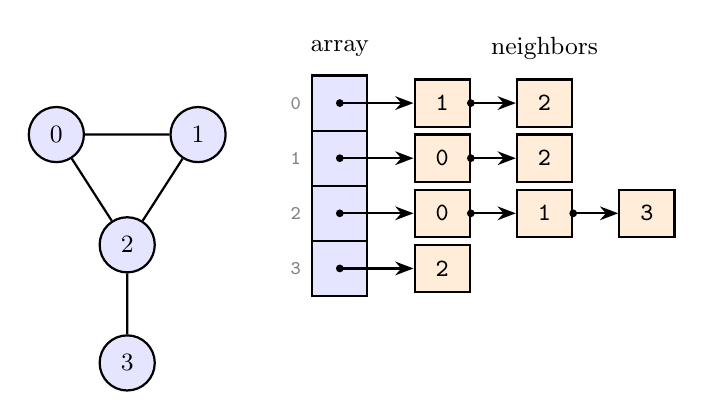
\begin{tikzpicture}[>={Stealth}, thick,
    v/.style={circle, draw, fill=blue!10, minimum size=7mm, font=\small},
    cell/.style={draw, minimum width=7mm, minimum height=7mm, font=\ttfamily\small},
    item/.style={draw, fill=orange!15, minimum width=7mm, minimum height=6mm, font=\ttfamily\small}]
  \node[v] (0) at (0,2) {0};
  \node[v] (1) at (1.8,2) {1};
  \node[v] (2) at (0.9,0.6) {2};
  \node[v] (3) at (0.9,-0.9) {3};
  \draw (0) -- (1) (0) -- (2) (1) -- (2) (2) -- (3);
  % Row r of the array sits at y = 2.4 - 0.7r; each neighbor list runs to its right
  \foreach \r/\list in {0/{1,2}, 1/{0,2}, 2/{0,1,3}, 3/{2}} {
    \node[cell, fill=blue!10, label={[font=\scriptsize\ttfamily, gray]left:\r}] (a\r) at (3.6,{2.4 - 0.7*\r}) {};
    \coordinate (prev) at (a\r.center);
    \foreach \n [count=\k] in \list {
      \node[item] (b) at ({3.6 + 1.3*\k},{2.4 - 0.7*\r}) {\n};
      \draw[->] (prev) -- (b.west);
      \fill (prev) circle (1.4pt);
      \coordinate (prev) at (b.east);
    }
  }
  \node[above=1mm of a0, font=\small] {array};
  \node[font=\small] at (6.2,3.1) {neighbors};
\end{tikzpicture}
